\documentclass[11pt]{article}
\usepackage{matt}
\begin{document}

\section*{Update for the Week of \today}

\begin{figure}[h]
  \centering
  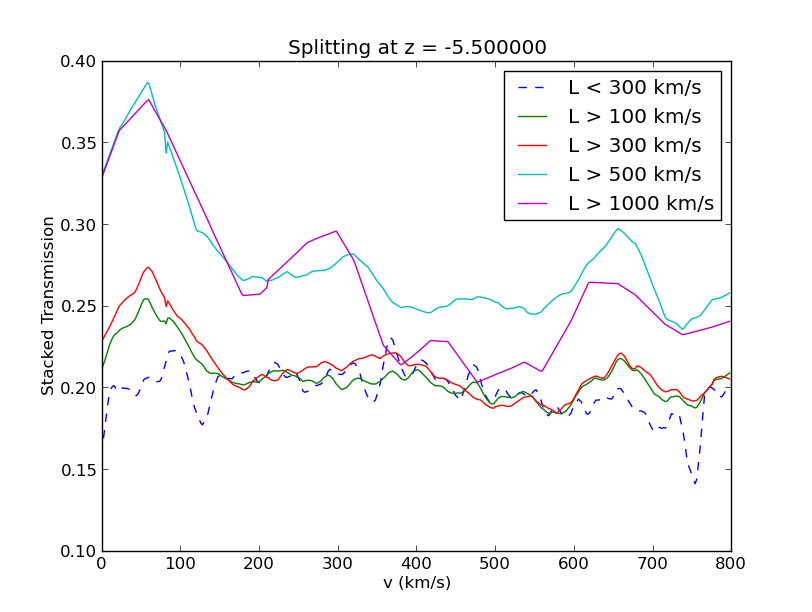
\includegraphics[width=7cm]{Stack_Zlessthan5p5.png}
  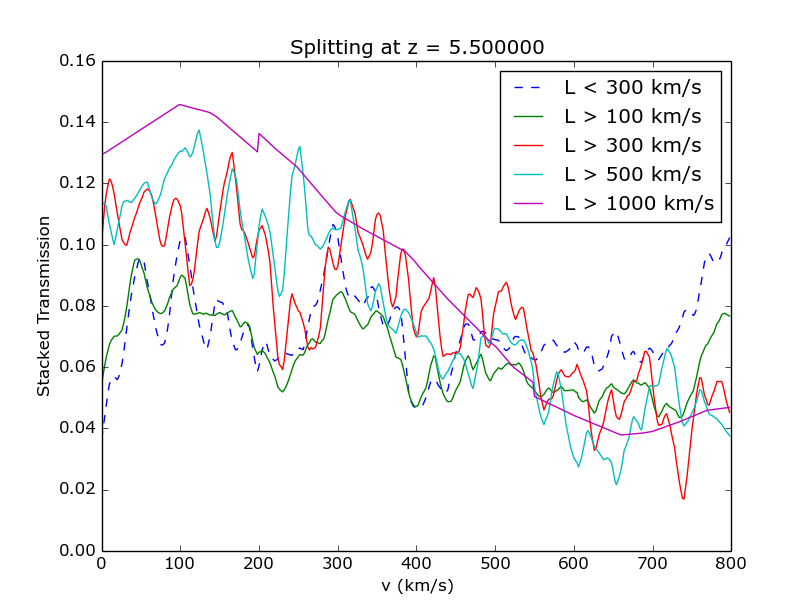
\includegraphics[width=7cm]{Stack_Zgreaterthan5p5.png}
  \caption{The above plots show the results of stacking outside of dark gaps located at $z \leq 5.5$ (left) and $z \geq 5.5$ (right). The first thing we notice is that the $z \geq 5.5$ plot is noisier but does not show a hint of a damping-wing feature. Additionally, we see that $\langle F \rangle_{z\leq 5.5} \approx 0.2$, while $\langle F \rangle_{z\geq 5.5} \approx 0.07$, somewhat consistent with what we'd expect.}
  \label{fig:z5p5}
\end{figure}

\begin{figure}[h]
  \centering
  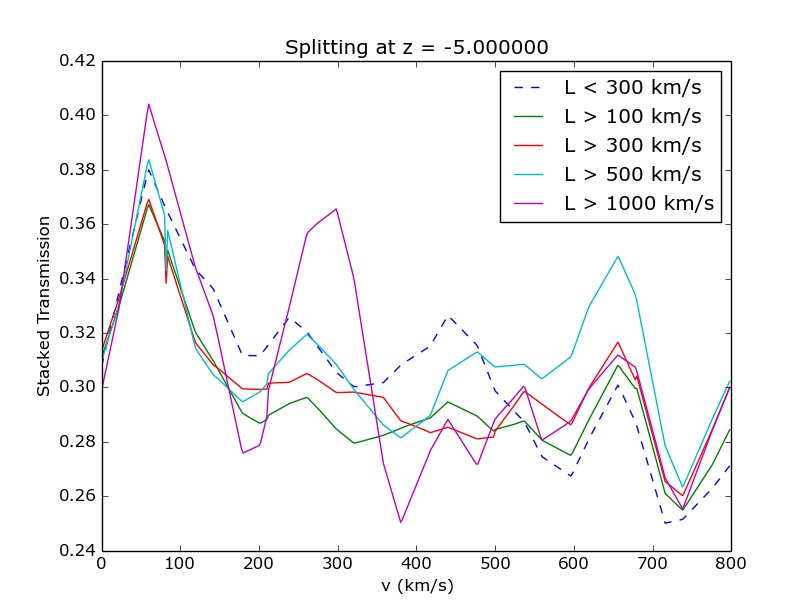
\includegraphics[width=7cm]{Stack_Zlessthan5.png}
  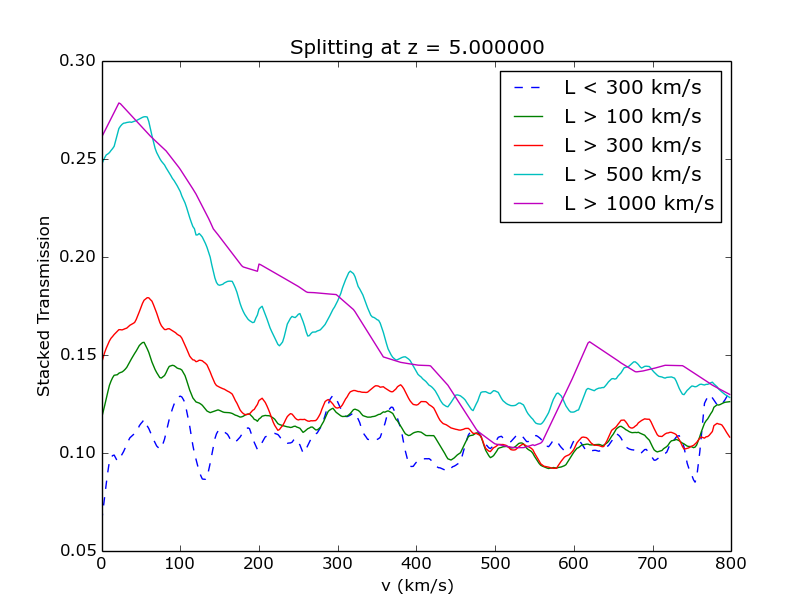
\includegraphics[width=7cm]{Stack_Zgreaterthan5.png}
  \caption{This figure is identical to Fig. \ref{fig:z5p5} except that we split the stacking at $z_{\text{cut}} = 5$ instead of $z_{\text{cut}} = 5.5$. By doing so, we see that we get $\langle F \rangle_{z>5} \approx 0.1$, somewhat matching what we would expect. It seems the curiously high mean transmission in the left-hand plot of Fig \ref{fig:z5p5} may be due to spectra at $z < 5$.}
  \label{fig:todo}
\end{figure}

\begin{figure}[h]
  \centering
  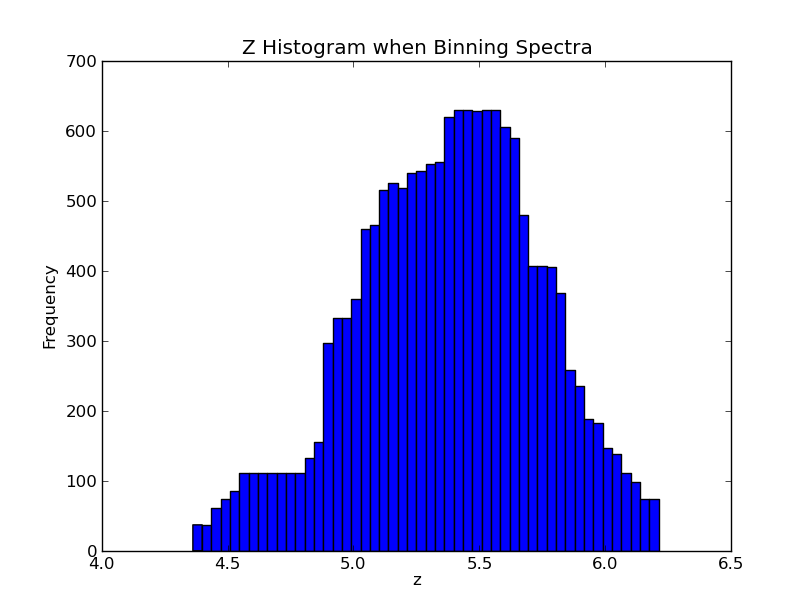
\includegraphics[width=8cm]{zHist_binned.png}
  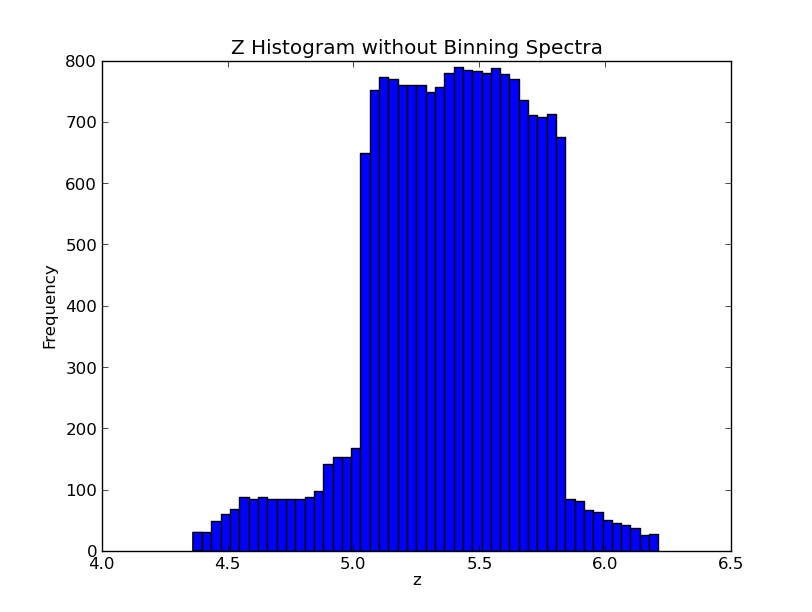
\includegraphics[width=8cm]{zHist_unbinned.png}
  \caption{The above figure shows the distribution of $z$ values that the pixels in our spectra take. The left-hand plot show the results when all spectra are binned to a common resolution, such that high-resolution spectra don't dominate the histogram, and the right-hand plot does not perform such a binning.}
  \label{fig:todo}
\end{figure}

\begin{figure}[h]
  \centering
  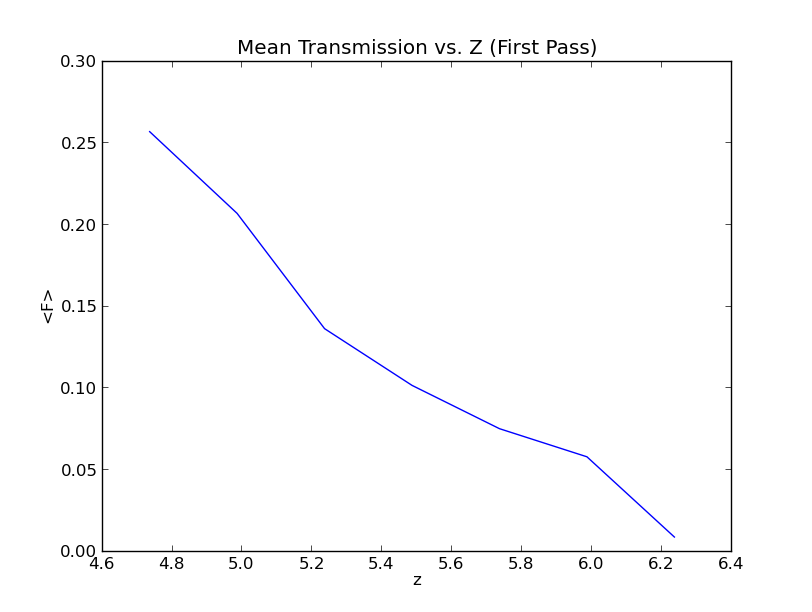
\includegraphics[width=8cm]{FvsZ.png}
  \caption{Mean transmission in \lya\ as a function of redshift for the spectra. Here we have bins in redshift of width $\Delta z = 0.25$ centered at $z$.}
  \label{fig:todo}
\end{figure}


\begin{figure}[h]
  \centering
  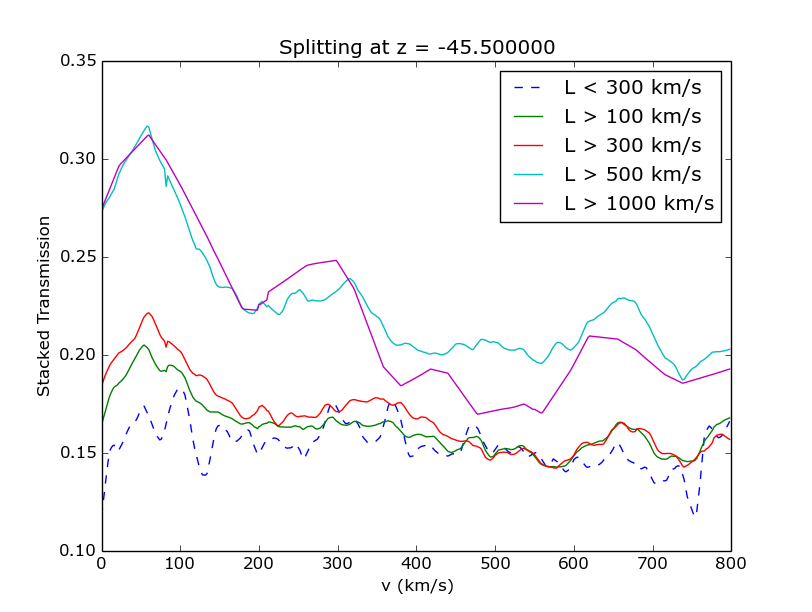
\includegraphics[width=8cm]{Stack_SanityCut.png}
  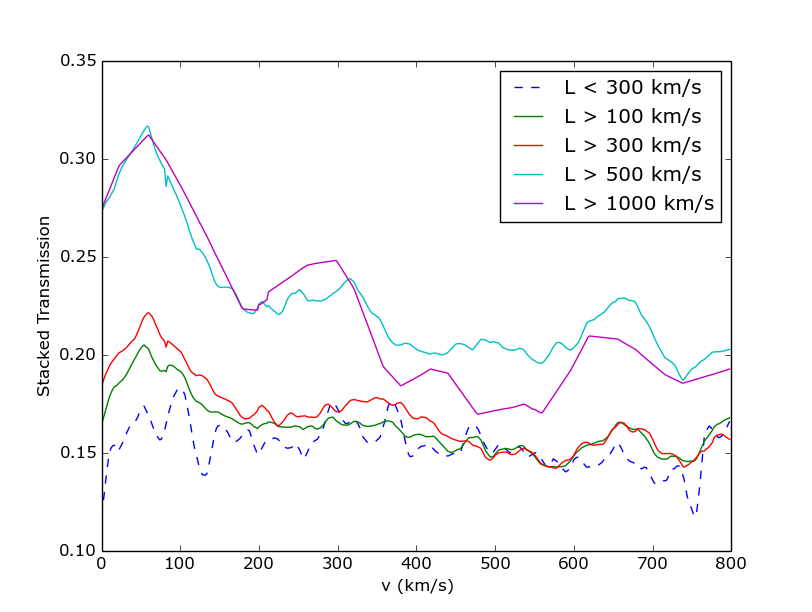
\includegraphics[width=8cm]{Stack_SanityCutCorrect.png}
  \caption{This is a sanity check, the two above plots should be the same.}
  \label{fig:todo}
\end{figure}


\end{document}